\PassOptionsToPackage{xetex}{xcolor}
\PassOptionsToPackage{xetex}{graphicx}
\documentclass[a4paper,landscape,headrule,footrule,xetex]{foils}

%%
%%% macros for 2009 Semester 1 HG 803
%%%
\newcommand{\logo}{~}
\newcommand{\header}[3]{%
  \title{\vspace*{-2ex} \large HG3051  Corpus Linquistics
    \\[2ex] \Large  \emp{#2} \\ \emp{#3}}
  \author{\blu{Francis Bond}   \\ 
    \normalsize  \textbf{Division of Linguistics and Multilingual Studies}\\
    \normalsize  \url{http://www3.ntu.edu.sg/home/fcbond/}\\
    \normalsize  \texttt{bond@ieee.org}}
  \MyLogo{HG3051 (2018)}
  \renewcommand{\logo}{#2}
  \hypersetup{
    pdfinfo={
      Author={Francis Bond},
      Title={#1: #2},
      Subject={HG3051: Corpus Linguistics},
      Keywords={Corpus Linguistics},
      License={CC BY 4.0}
    }
  }
  \date{#1 \\ \url{https://github.com/bond-lab/Corpus-Linguistics}}
}

\usepackage{fontenc}
\usepackage{polyglossia}
\setmainlanguage{english}
\setmainfont{TeX Gyre Pagella}
%\setmainfont{Linux Libertine}
%\setmainfont{Charis SIL}
\newfontfamily{\ipafont}{Gentium}
\newcommand{\ipa}[1]{{\ipafont\selectfont #1}}
\usepackage{xeCJK}

\setCJKmainfont{Noto Sans CJK SC}
\setCJKsansfont{Noto Sans CJK SC}



\usepackage{xcolor}
\usepackage{graphicx}
\newcommand{\blu}[1]{\textcolor{blue}{#1}}
\newcommand{\grn}[1]{\textcolor{green}{#1}}
\newcommand{\hide}[1]{\textcolor{white}{#1}}
\newcommand{\emp}[1]{\textcolor{red}{#1}}
\newcommand{\txx}[1]{\textbf{\textcolor{blue}{#1}}}
\newcommand{\lex}[1]{\textbf{\mtcitestyle{#1}}}

\usepackage{pifont}
\renewcommand{\labelitemi}{\textcolor{violet}{\ding{227}}}
\renewcommand{\labelitemii}{\textcolor{purple}{\ding{226}}}

\newcommand{\subhead}[1]{\noindent\textbf{#1}\\[5mm]}

\newcommand{\Bad}{\emp{\raisebox{0.15ex}{\ensuremath{\mathbf{\otimes}}}}}
\newcommand{\bad}{*}

\newcommand{\com}[1]{\hfill \textnormal{(\emp{#1})}}%
\newcommand{\cxm}[1]{\hfill \textnormal{(\txx{#1})}}%
\newcommand{\cmm}[1]{\hfill \textnormal{(#1)}}%

\usepackage{relsize,xspace}
\newcommand{\into}{\ensuremath{\rightarrow}\xspace}
\newcommand{\ent}{\ensuremath{\Rightarrow}\xspace}
\newcommand{\nent}{\ensuremath{\not\Rightarrow}\xspace}
\newcommand{\tot}{\ensuremath{\leftrightarrow}\xspace}
\usepackage{url}
\newcommand{\lurl}[1]{\MyLogo{\url{#1}}}

\usepackage{mygb4e}
\let\eachwordone=\itshape
\newcommand{\lx}[1]{\textbf{\textit{#1}}}

%\usepackage{times}
%\usepackage{nttfoilhead}
\newcommand{\myslide}[1]{\foilhead[-25mm]{\raisebox{12mm}[0mm]{\emp{#1}}}\MyLogo{\logo}}
\newcommand{\myslider}[1]{\rotatefoilhead[-25mm]{\raisebox{12mm}[0mm]{\emp{#1}}}}
%\newcommand{\myslider}[1]{\rotatefoilhead{\raisebox{-8mm}{\emp{#1}}}}

\newcommand{\section}[1]{\myslide{}{\begin{center}\Huge \emp{#1}\end{center}}}



\usepackage[lyons,j,e,k]{mtg2e}
\renewcommand{\mtcitestyle}[1]{\textcolor{teal}{\textsl{#1}}}
%\renewcommand{\mtcitestyle}[1]{\textsl{#1}}
\newcommand{\chn}{\mtciteform}
\newcommand{\cmn}{\mtciteform}
\newcommand{\iz}[1]{\textup{\texttt{\textcolor{blue}{\textbf{#1}}}}}
\newcommand{\rel}[1]{\textsc{\color{blue}{#1}}}
\newcommand{\wn}[3]{\lex{#1}\ensuremath{_{#2:#3}}}
\newcommand{\con}[1]{\textsc{#1}}
\newcommand{\gm}{\textsc}
\usepackage[normalem]{ulem}
\newcommand{\ul}{\uline}
\newcommand{\ull}{\uuline}
\newcommand{\wl}{\uwave}
\newcommand{\vs}{\ensuremath{\Leftrightarrow}~}
\usepackage[hidelinks]{hyperref}
\hypersetup{
     colorlinks,
     linkcolor={blue!50!black},
     citecolor={red!50!black},
     urlcolor={blue!80!black}
}
%%%
%%% Bibliography
%%%
\usepackage{natbib}
%\usepackage{url}
\usepackage{bibentry}
%%% From Tim
\newcommand{\WMngram}[1][]{$n$-gram#1\xspace}
\newcommand{\infers}{$\rightarrow$\xspace}


\header{Multimodal and Multilingual Corpora}{}

\usepackage{pst-node}
\newcommand{\sa}[2]{\rnode{c#1}{\iz{#2}}}%\nodebox{c#1}}

%\usepackage{hieroglf}
\usepackage{wasysym}

\begin{document}
\bibliographystyle{apalike}
\nobibliography{abb,mtg,nlp,ling}
\maketitle


\myslide{Overview}

\begin{itemize} 
\item Revision of Annotation
  \begin{itemize}
  \item \blu{Mark-up}
  \item \blu{Annotation}
  \item \blu{Regular Expressions}
  \end{itemize}
\item \blu{Multi-modal Corpora}
\item \blu{Multi-lingual Corpora}
\end{itemize}


%%%
\section{Revision of Annotation}
%%%

\myslide{Corpus Annotation vs. Mark-Up}
  \begin{itemize}
  \item \txx{Mark up} provides objectively verifiable information
    \begin{itemize}
    \item Authorship
    \item Publication dates
    \item Paragraph boundaries
    \item Source text (URL, Book, \ldots)
    \item License
    \end{itemize}
  \item \txx{Annotation} provides interpretive linguistic information
    \begin{itemize}
    \item Sentence/Utterance boundaries
    \item Tokenization
    \item Part-of-speech tags, Lemmas, Concepts
    \item Sentence structure (syntax, co-reference, roles)
    \item Domain, Genre
    \end{itemize}
  \end{itemize}

\myslide{Dublin Core Ontology}
\MyLogo{\url{http://dublincore.org/}}
\begin{itemize}
\item Goals
  \begin{itemize}
  \item Provides a semantic vocabulary for describing the
    ``core'' information properties of resources (electronic
    and ``real'' physical objects)
  \item Enables intelligent resource discovery systems
  \end{itemize}
\item Fifteen Elements:
  \begin{itemize}
  \item Content (7)
    \begin{itemize}
    \item Title, Subject, Description, Type, Source,
      Relation and Coverage
    \end{itemize}
  \item Intellectual property (4)
    \begin{itemize}
    \item Creator, Publisher, Contributor, Rights
    \end{itemize}
  \item Instantiation (4)
    \begin{itemize}
    \item Date, Language, Format, Identifier
    \end{itemize}
  \end{itemize}
\item \blu{OLAC Lang. Resource Catalog}: {\small \url{http://search.language-archives.org/}}
\end{itemize}



\myslide{Geoffrey Leech's Seven Maxims of Annotation}
\MyLogo{}
\begin{enumerate}
\item Annotation should be separable from text, leaving the raw corpus.
\item It should be possible to extract just the annotations
from the text. 
\item The annotation guidelines should be available.
\item Who did the annotation and how should be made clear.
\item The possibilities of errors should be made clear.
\item Annotation schemes should be theory-neutral 
\item Standards emerge through practical consensus.
\end{enumerate}

\myslide{Types of Corpus Annotation}
\begin{itemize}
\item  Tokenization, Lemmatization
\item  Part-of-speech
\item  Syntactic analysis (chunks, parses)
\item  Semantic analysis  (word senses, semantic roles)
\item  Discourse and pragmatic analysis (co-reference, time)
\item  Phonetic, phonemic, prosodic annotation
\item  Error tagging
\end{itemize}

\myslide{How is Corpus Annotation Done?}
\begin{itemize}
\item Mainly semi-automatic (done first by computer programs; post-edited)
 \begin{enumerate}
  \item An small annotated corpus is built, entirely by humans
  \item Then a computer program is \txx{trained} on this corpus
  \item Now new corpora can be automatically annotated using this program
  \end{enumerate}
\item Large corpora often fully automatic
  \begin{itemize}
  \item Segmentation
  \item Part-of-speech tagging: accuracy of 97\%
  \item Lemmatization
  \end{itemize}
\item Corpora should indicate reliability of tags
  \begin{itemize}
  \item Inter-annotator agreement, kappa (human)
  \item Tagger accuracy (machine)
  \end{itemize}
  
\end{itemize}


\myslide{How are corpora represented?}

\begin{itemize}
\item Far too many encoding schemes (TEI is common)
  \begin{itemize}
  \item Header: for mark up
  \item Body: for annotation
  \end{itemize}
\item Text: one sentence per line, POS affixed \texttt{can\_VV}
\item XML: \texttt{<s sid='1'><w wid = '1' pos='vv'>can</w></s>}
\item XML standoff: 
  \\ can \hfill (text file)
  \\ \texttt{<w pos='vv' cfrom='0' cto='3' />} \hfill (corpus file)
\item Often stored in a database in applications

\end{itemize}

\myslide{Best Practices}

\begin{itemize}
\item XML
\item Header and documentation
\item Open license
\item Maintained (errors corrected, dynamic updates)
\end{itemize}

% \myslide{Case Study: the Hinoki Corpus}

% \begin{itemize}
% \item Grammar-based syntactic annotation using discriminants
%   \begin{itemize}
%   \item Parse the corpus and select the best parse
%     \begin{itemize}
%     \item discriminant-based selection is efficient
%     \end{itemize}
%   \item Guarantees consistency
%   \item Loses some trees
%   \end{itemize}
% \end{itemize}
% \myslide{Discriminant-based Treebanking}
% \begin{itemize}
% \item Calculate \emp{elementary discriminants} (Carter 1997)
%   \begin{itemize}
%   \item Basic contrasts between parses
%   \item Mostly independent and local
%   \item Can be syntactic or semantic
%   \end{itemize}
% \item Select or reject discriminants until one parse remains
%   \begin{itemize}
%   \item $|{\textnormal{decisions}| \propto \log |\textnormal{parses}|}$
%   \end{itemize}
% \item Alternatively reject all parses
%   \begin{itemize}
%   \item i.e, the grammar can not parse successfully
%   \end{itemize}
% \end{itemize}



% \myslide{Derivations of \jpn[curtain]{k\=aten}$_2$ (4/6)}

% \vspace*{-3mm}{\tiny
%  \hspace*{-15mm}\begin{tabular}{c@{\,}c} 

%   \addtolength{\tabcolsep}{-0.3em}
%   \begin{tabular}{ccccccc}
%    &\multicolumn{5}{c}{\sa{1}{NP-frag}}  \\[1ex]
%    &\multicolumn{5}{c}{\sa{2}{\wl{rel-cl-sbj-gap}}}  \\[1ex]
%    &\multicolumn{3}{c}{\sa{3}{hd-complement}} & \sa{4}{N} \\[1ex]
%    \multicolumn{3}{c}{\sa{5}{hd-complement}} & \multicolumn{1}{c}{\sa{J}{V}} &
%    \\[1ex]
%    \multicolumn{2}{c}{\sa{I}{\ul{hd-specifier}}} & & &  & \\[1ex]
%    \sa{H}{DET} & \sa{7}{N}      & \sa{8}{CASE-P} &   &  \\[1ex]
%    %N      & &  &  V &  \\   
%    \sa{G}{ある} & \sa{B}{物事} & \sa{C}{を} & \sa{D}{隠す} &  \sa{F}{ 物} \\
%    \texttt{\emp{\ul{adnominal}}} & \texttt{noun} & \texttt{particle} & \texttt{verb} & \texttt{noun} \\
%    a certain & thing &  \textsc{acc} & hide &  thing \\
%    \multicolumn{5}{c}{Tree \#1 (Correct)} \\ \\
%   \end{tabular}
%   \centering
%   \ncline[nodesep=3pt]{c1}{c2} \ncline[nodesep=3pt]{c2}{c3}
%   \ncline[nodesep=3pt]{c2}{c4} \ncline[nodesep=3pt]{c3}{c5}
%   \ncline[nodesep=3pt]{cA}{c6} \ncline[nodesep=3pt]{c4}{cF}
%   \ncline[nodesep=3pt]{c5}{c8}
%   \ncline[nodesep=3pt]{cJ}{c3} \ncline[nodesep=3pt]{cI}{c5} 
%   \ncline[nodesep=3pt]{c7}{cI} \ncline[nodesep=3pt]{c8}{cC}
%   \ncline[nodesep=3pt]{cG}{cH} \ncline[nodesep=3pt]{cH}{cI}
%   \ncline[nodesep=3pt]{cD}{cJ} 
%   \ncline[nodesep=3pt]{cB}{c7} 
%   %\caption{Derivation Tree \#1 of the Definition of カーテン$_2$ \jpn[curtain]{k\=aten}}
%   %  \label{fig:derivation-curtain-1}
% %\end{figure}
  
%   %\begin{figure}[htbp]
%   %  \centering
%   %\addtolength{\tabcolsep}{-0.3em}
%   %\vspace{3mm}
%   &
%   \begin{tabular}{ccccccc}
%     &\multicolumn{5}{c}{\sa{1}{NP-frag}}  \\[1ex]
%     &\multicolumn{5}{c}{\sa{2}{\wl{rel-clause}}}  \\[1ex]
%     &\multicolumn{3}{c}{\sa{3}{hd-complement}} & \sa{4}{N} \\[1ex]
%     \multicolumn{3}{c}{\sa{5}{hd-complement}} & \multicolumn{1}{c}{\sa{J}{\wl{subj-zpro}}} &
%     \\[1ex]
%     \multicolumn{2}{c}{\sa{I}{\ul{hd-specifier}}} & & \sa{K}{V} & & \\[1ex]
%     \sa{H}{DET} & \sa{7}{N}      & \sa{8}{CASE-P} &   &  \\[1ex]
%                                 %N      & &  &  V &  \\   
%     \sa{G}{ある} & \sa{B}{物事} & \sa{C}{を} & \sa{D}{隠す} &  \sa{F}{ 物} \\
%    \texttt{\emp{\ul{adnominal}}} & \texttt{noun} & \texttt{particle} & \texttt{verb} & \texttt{noun} \\
%     a certain & thing &  \textsc{acc} & hide &  thing \\
%    \multicolumn{5}{c}{Tree \#2} \\ \\
%   \end{tabular}\\
%   \centering
%   \ncline[nodesep=3pt]{c1}{c2} \ncline[nodesep=3pt]{c2}{c3}
%   \ncline[nodesep=3pt]{c2}{c4} \ncline[nodesep=3pt]{c3}{c5}
%   \ncline[nodesep=3pt]{cA}{c6} \ncline[nodesep=3pt]{c4}{cF}
%   \ncline[nodesep=3pt]{c5}{c8}
%   \ncline[nodesep=3pt]{cJ}{c3} \ncline[nodesep=3pt]{cI}{c5} 
%   \ncline[nodesep=3pt]{c7}{cI} \ncline[nodesep=3pt]{c8}{cC}
%   \ncline[nodesep=3pt]{cG}{cH} \ncline[nodesep=3pt]{cH}{cI}
%   \ncline[nodesep=3pt]{cD}{cK} \ncline[nodesep=3pt]{cK}{cJ} 
%   \ncline[nodesep=3pt]{cB}{c7} 

%   %\label{fig:derivation-curtain-2}
%    %\end{figure}

%  \begin{tabular}{ccccccc}
%     &\multicolumn{5}{c}{\sa{1}{NP-frag}}  \\[1ex]
%     &\multicolumn{5}{c}{\sa{2}{\wl{rel-cl-sbj-gap}}}  \\[1ex]
%     &\multicolumn{3}{c}{\sa{3}{hd-complement}} & \sa{4}{N} \\[1ex]
%     \multicolumn{3}{c}{\sa{5}{hd-complement}} & \multicolumn{1}{c}{\sa{J}{V}} &
%     \\[1ex]
%     \multicolumn{2}{c}{\sa{I}{\ul{rel-cl-sbj-gap}}} & & &  & \\[1ex]
%     \sa{H}{V} & \sa{7}{N}      & \sa{8}{CASE-P} &   &  \\[1ex]
%                                 %N      & &  &  V &  \\   
%     \sa{G}{ある} & \sa{B}{物事} & \sa{C}{を} & \sa{D}{隠す} &  \sa{F}{ 物} \\
%    \texttt{\emp{\ul{verb}}} & \texttt{noun} & \texttt{particle} & \texttt{verb} & \texttt{noun} \\
%     exist & thing &  \textsc{acc} & hide &  thing \\
%    \multicolumn{5}{c}{Tree \#3} \\ \\
%  \end{tabular}
%   \centering
%   \ncline[nodesep=3pt]{c1}{c2} \ncline[nodesep=3pt]{c2}{c3}
%   \ncline[nodesep=3pt]{c2}{c4} \ncline[nodesep=3pt]{c3}{c5}
%   \ncline[nodesep=3pt]{cA}{c6} \ncline[nodesep=3pt]{c4}{cF}
%   \ncline[nodesep=3pt]{c5}{c8}
%   \ncline[nodesep=3pt]{cJ}{c3} \ncline[nodesep=3pt]{cI}{c5} 
%   \ncline[nodesep=3pt]{c7}{cI} \ncline[nodesep=3pt]{c8}{cC}
%   \ncline[nodesep=3pt]{cG}{cH} \ncline[nodesep=3pt]{cH}{cI}
%   \ncline[nodesep=3pt]{cD}{cJ} 
%   \ncline[nodesep=3pt]{cB}{c7} 
% % \caption{Derivation Tree \#3 of the Definition of カーテン$_2$ \jpn[curtain]{k\=aten}}
% %  \label{fig:derivation-curtain-3}
% %\end{figure}

% %\begin{figure}[htbp]
% %  \centering
% %\addtolength{\tabcolsep}{-0.3em}

% &
%   \begin{tabular}{ccccccc}
%     &\multicolumn{5}{c}{\sa{1}{NP-frag}}  \\[1ex]
%     &\multicolumn{5}{c}{\sa{2}{\wl{rel-clause}}}  \\[1ex]
%     &\multicolumn{3}{c}{\sa{3}{hd-complement}} & \sa{4}{N} \\[1ex]
%     \multicolumn{3}{c}{\sa{5}{hd-complement}} & \multicolumn{1}{c}{\sa{J}{\wl{subj-zpro}}} &
%     \\[1ex]
%     \multicolumn{2}{c}{\sa{I}{\ul{rel-cl-sbj-gap}}} & & \sa{K}{V} &  & \\[1ex]
%     \sa{H}{V} & \sa{7}{N}      & \sa{8}{CASE-P} &   &  \\[1ex]
%                                 %N      & &  &  V &  \\   
%     \sa{G}{ある} & \sa{B}{物事} & \sa{C}{を} & \sa{D}{隠す} &  \sa{F}{ 物} \\
%    \texttt{\emp{\ul{verb}}} & \texttt{noun} & \texttt{particle} & \texttt{verb} & \texttt{noun} \\
%     exist & thing &  \textsc{acc} & hide &  thing \\
%    \multicolumn{5}{c}{Tree \#4} \\ \\
%   \end{tabular}
%   \ncline[nodesep=3pt]{c1}{c2} \ncline[nodesep=3pt]{c2}{c3}
%   \ncline[nodesep=3pt]{c2}{c4} \ncline[nodesep=3pt]{c3}{c5}
%   \ncline[nodesep=3pt]{cA}{c6} \ncline[nodesep=3pt]{c4}{cF}
%   \ncline[nodesep=3pt]{c5}{c8}
%   \ncline[nodesep=3pt]{cJ}{c3} \ncline[nodesep=3pt]{cI}{c5} 
%   \ncline[nodesep=3pt]{c7}{cI} \ncline[nodesep=3pt]{c8}{cC}
%   \ncline[nodesep=3pt]{cG}{cH} \ncline[nodesep=3pt]{cH}{cI}
%   \ncline[nodesep=3pt]{cD}{cK} \ncline[nodesep=3pt]{cK}{cJ} 
%   \ncline[nodesep=3pt]{cB}{c7} 
% % \caption{Derivation Tree \#4 of the Definition of カーテン$_2$ \jpn[curtain]{k\=aten}}
% %  \label{fig:derivation-curtain-4}
% %\end{figure}

% %\begin{figure}[htbp]
% %  \centering
% %\addtolength{\tabcolsep}{-0.3em}
% %\vspace{3mm}

% %   \begin{tabular}{ccccccc}
% %     &\multicolumn{5}{c}{\sa{1}{NP-frag}}  \\[1ex]
% %     &\multicolumn{5}{c}{\sa{2}{rel-cl-sbj-gap}}  \\[1ex]
% %     &\multicolumn{3}{c}{\sa{3}{hd-complement}} & \sa{4}{N} \\[1ex]
% %     \multicolumn{3}{c}{\sa{5}{hd-complement}} & \multicolumn{1}{c}{\sa{J}{V}} &
% %     \\[1ex]
% %     \multicolumn{2}{c}{\sa{I}{rel-clause}} & & &  & \\[1ex]
% %     \sa{L}{subj-zpro} &        &  &   &  \\[1ex]
% %     \sa{H}{V} & \sa{7}{N}      & \sa{8}{CASE-P} &   &  \\[1ex]
% %                                 %N      & &  &  V &  \\   
% %     \sa{G}{ある} & \sa{B}{物事} & \sa{C}{を} & \sa{D}{隠す} &  \sa{F}{ 物} \\
% %    \texttt{\ul{verb}} & \texttt{noun} & \texttt{particle} & \texttt{verb} & \texttt{noun} \\
% %     exist & thing &  \textsc{acc} & hide &  thing \\
% %    \multicolumn{5}{c}{Tree \#5} \\ \\
% %   \end{tabular}
% %   \centering
% %   \ncline[nodesep=3pt]{c1}{c2} \ncline[nodesep=3pt]{c2}{c3}
% %   \ncline[nodesep=3pt]{c2}{c4} \ncline[nodesep=3pt]{c3}{c5}
% %   \ncline[nodesep=3pt]{cA}{c6} \ncline[nodesep=3pt]{c4}{cF}
% %   \ncline[nodesep=3pt]{c5}{c8}
% %   \ncline[nodesep=3pt]{cJ}{c3} \ncline[nodesep=3pt]{cI}{c5} 
% %   \ncline[nodesep=3pt]{c7}{cI} \ncline[nodesep=3pt]{c8}{cC}
% %   \ncline[nodesep=3pt]{cG}{cH} \ncline[nodesep=3pt]{cH}{cL} \ncline[nodesep=3pt]{cL}{cI}
% %   \ncline[nodesep=3pt]{cD}{cJ} \ncline[nodesep=3pt]{c7}{cB} 
% % % \caption{Another Derivation Tree \#5 of the Definition of カーテン$_2$ \jpn[curtain]{k\=aten}}
% % %  \label{fig:derivation-curtain-5}
% % %\end{figure}

% % %\begin{figure}[htbp]
% % %  \centering
% % %\addtolength{\tabcolsep}{-0.3em}
% % %\vspace{3mm}
% % &
% %   \begin{tabular}{ccccccc}
% %     &\multicolumn{5}{c}{\sa{1}{NP-frag}}  \\[1ex]
% %     &\multicolumn{5}{c}{\sa{2}{rel-clause}}  \\[1ex]
% %     &\multicolumn{3}{c}{\sa{3}{hd-complement}} & \sa{4}{N} \\[1ex]
% %     \multicolumn{3}{c}{\sa{5}{hd-complement}} & \multicolumn{1}{c}{\sa{J}{subj-zpro}} &
% %     \\[1ex]
% %     \multicolumn{2}{c}{\sa{I}{rel-clause}} & & \sa{K}{V} &  & \\[1ex]
% %     \sa{L}{subj-zpro} &        &  &   &  \\[1ex]
% %     \sa{H}{V} & \sa{7}{N}      & \sa{8}{CASE-P} &   &  \\[1ex]
% %                                 %N      & &  &  V &  \\   
% %     \sa{G}{ある} & \sa{B}{物事} & \sa{C}{を} & \sa{D}{隠す} &  \sa{F}{ 物} \\
% %    \texttt{\ul{verb}} & \texttt{noun} & \texttt{particle} & \texttt{verb} & \texttt{noun} \\
% %     exist & thing &  \textsc{acc} & hide &  thing \\
% %    \multicolumn{5}{c}{Tree \#6} \\ \\
% %   \end{tabular}
% %   \centering
% %   \ncline[nodesep=3pt]{c1}{c2} \ncline[nodesep=3pt]{c2}{c3}
% %   \ncline[nodesep=3pt]{c2}{c4} \ncline[nodesep=3pt]{c3}{c5}
% %   \ncline[nodesep=3pt]{cA}{c6} \ncline[nodesep=3pt]{c4}{cF}
% %   \ncline[nodesep=3pt]{c5}{c8}
% %   \ncline[nodesep=3pt]{cJ}{c3} \ncline[nodesep=3pt]{cI}{c5} 
% %   \ncline[nodesep=3pt]{c7}{cI} \ncline[nodesep=3pt]{c8}{cC}
% %   \ncline[nodesep=3pt]{cG}{cH} \ncline[nodesep=3pt]{cH}{cL} \ncline[nodesep=3pt]{cL}{cI}
% %   \ncline[nodesep=3pt]{cD}{cK} \ncline[nodesep=3pt]{cK}{cJ}
% %  \ncline[nodesep=3pt]{c7}{cB} 
%  \end{tabular}
% }
% \vspace*{-20mm}


% \myslide{Hinoki --- Summary}

% \begin{itemize}
% \item  5,000 sentences are annotated by three different annotators
% \item  average inter-annotator agreement
%   \begin{itemize}
%   \item 65.4\% (sentence)
%   \item 83.5\% using labeled precision
%     \\ bracket with same label in the same place
%   \item 96.6\% on ambiguous annotated trees 
%     \\ most disagreement is in if the tree is good or not
%   \end{itemize}
% \item Hinoki corpus was then extended to another 30,000 trees
% \end{itemize}



\section{Multi-Modal Corpora}

\myslide{Multi-modal Corpora}

\begin{itemize}
\item Language is not the only channel for communication: It is often
  combined with other modalities
  \begin{itemize}
  \item speech
  \item gesture
  \item facial expression
  \item gaze
  \item body posture
\\ ECG (Electrocardiogram), HR (Heart Rate), GSR (Galvanic Skin Response)
  \item activity: nursing, drawing, building
  \item orthographic cues (color, size, font choice, \ldots)
  \end{itemize}
\item Corpora that include more than one of these are \blu{multi-modal}
\end{itemize}

\myslide{HCRC Map Task}
\MyLogo{\url{http://groups.inf.ed.ac.uk/maptask/}}
\begin{itemize}
\item Early, influential dialog corpus (with maps)
\item Task
  \begin{itemize}
  \item Two speakers sit opposite one another
  \item Each has a map which the other cannot see
  \item The Instruction Giver has a route marked on their map
  \item The Instruction Follower has no route
  \item The goal is to reproduce the Instruction Giver's route on the Instruction Follower's map
  \item The maps are not identical and the speakers are told this
  \end{itemize}
\item Conditions
  \begin{itemize}
  \item familiar (friends) vs non-familiar
  \item gaze vs no-gaze
  \end{itemize}
\end{itemize}

\myslide{The Maps}

\begin{center}
  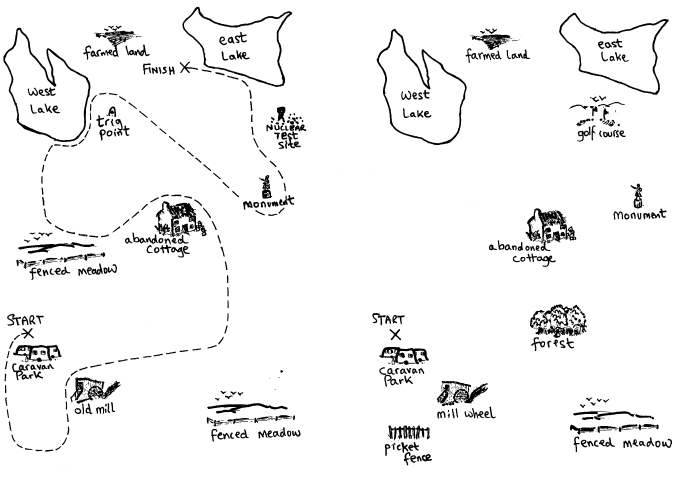
\includegraphics[width=0.75\textwidth]{include/maps}
\end{center}

\myslide{Some design points}

\begin{itemize}
\item Landmarks chosen for phonetic properties
  \begin{itemize}
\item /t/-deletion eg \textit{vast meadow}
\item /d/-deletion eg \textit{reclaimed fields}
\item glottalisation eg \textit{chestnut tree}
\item nasal assimilation eg \textit{broken gate }
\end{itemize}
Making the data maximally useful
\item Annotation
  \begin{itemize}
  \item POS, parse
  \item Discourse structure
  \item Gaze
  \end{itemize}
\item Now replicated in many languages and dialects (Dutch, Italian, Japanese, Swedish, Occitan, Portuguese, Australian, American and British English)
\end{itemize}

\myslide{E-Nightingale: Nursing Task Corpus}
\MyLogo{\url{https://aclanthology.org/I05-6005.pdf}}
\begin{itemize}
\item Japanese project to analyze Nursing tasks and dialogs
\item recorder worn all day
\item beeps at ten minute intervals  (event-driven recording)
  \begin{itemize}
  \item Nurse records what they are doing
  \end{itemize}
\item Linked to location
\item Very hard speech to decode
\end{itemize}
Hiromi Itoh Ozaku; Akinori Abe; Noriaki Kuwahara; Futoshi Naya; Kiyoshi Kogure; Kaoru Sagara
\textit{Building Dialogue Corpora for Nursing Activity Analysis} in LINC-2005



\myslide{VACE Multimodal Meeting Corpus}
\MyLogo{\url{https://www.researchgate.net/publication/225343582_VACE_multimodal_meeting_corpus}}

Lei Chen, R. Rose, Qiao Ying, Irene Kimbara, Fey Parrill, Haleema
Welji, Tony Han, Jilin Tu, Zhongqiang Huang, Mary Harper,
Francis Quek, Yingen Xiong, David Mcneill,  Ronald Tuttle and
Thomas Huang. (2006). VACE multimodal meeting
corpus. 40-51. \url{https://dx.doi.org/10.1007/11677482_4}

 \begin{itemize}
\item Industrial scale coding, 10 cameras, separate audio for each speaker:
  \begin{itemize}
  \item motion capture
  \item gaze
  \item speech automatic; OOV by experts; further checking
  \item detailed information about the participants
  \item detailed information about the task
  \end{itemize}
\end{itemize}


\myslide{British Sign Language Corpus}
\MyLogo{http://www.bslcorpusproject.org}

\begin{itemize}
\item Collection of sign language recordings (2008--2011)
  \begin{itemize}
  \item 249 deaf signers of BSL from 8 regions around the UK: 
    \\London (L), Bristol (BL), Cardiff (CF), Birmingham (BM), Newcastle (N), Manchester (M), Glasgow (G) and Belfast (BF).
  \item mixed for gender, age group, age of BSL acquisition, social class and ethnicity
  \item  interviews (i); conversation (c); narrative followed by conversation (n-c)
  \end{itemize}
\item Marked up with the above information
\item Gave rise to many new projects
  \begin{itemize}
  \item BSL SignBank
  \item Directional verbs
  \item BSL Syntax
  \item ExTOL: End to End Translation of British Sign Language
  \end{itemize}
\end{itemize}



\section{Multi-Lingual Corpora}
\MyLogo{}

\myslide{Bitexts and more}

\begin{itemize}
\item Multilingual corpora are useful for
  \begin{itemize}
  \item Contrastive linguistic analysis
    \begin{itemize}
    \item Comparing distributions between languages
    \item Learning about translations
    \item using one language to describe the other
    \end{itemize}
  \item Language learning
    \begin{itemize}
    \item Teaching new phenomena in terms of what you already know
    \end{itemize}
  \item Machine translation training
    \begin{itemize}
    \item Learning translations directly
    \end{itemize}
  \end{itemize}
\end{itemize}

%%% Fixme double matches
\myslide{Europarl}
\MyLogo{\url{http://www.statmt.org/europarl/}; \url{http://opus.lingfil.uu.se/cwb/Europarl7/frames-cqp.html}}

\begin{itemize}
\item Large automatically aligned corpus of European parliament proceedings
  \item Translation between EU languages (EU funded project)
  \item 18-40 million words, .6--1.3 million sentences
  \item Freely available text in all European Languages
  \item Used in the Euro Matrix MT project
\end{itemize}
\begin{quote}
  \textit{Europarl: A Parallel Corpus for Statistical Machine Translation}, Philipp Koehn, MT Summit 2005
\end{quote}



\myslide{Euro Matrix SMT Results}
  \MyLogo{}
\begin{center}
\rotatebox{180}{\includegraphics[angle=90,height=0.97\textheight]{include/euro-matrix.epsi}}
\end{center}

\myslide{Euro Matrix Discussion}

\begin{itemize}
\item Linguistic similarity affects the statistical machine translation score:
  \begin{itemize}
  \item Highest: Spanish \into French (BLEU = 40.27)
  \item Lowest: Italian \into Finnish  (BLEU = 11.08)
  \end{itemize}

\item Translation done using the open source SMT System:
 \\ \blu{Moses} \url{<statmt.org>}

\item Creating all $n(n-1)$ language pairs took a week
  \begin{itemize}
  \item It is easy to train new systems if you have a multi-lingual corpus
  \end{itemize}
\end{itemize}

\myslide{Interesting facts}

\begin{itemize}
\item Also used for lexicon and thesaurus construction
\item Several English on-line translations are actually French
  \\ and no-one had noticed 
\item Almost entirely constructed automatically
\item New languages being added to the EU means more data
\end{itemize}


\myslide{OPUS}
\MyLogo{\url{https://opus.nlpl.eu/}}

\begin{itemize}
\item On-line collection of multilingual text
\item Mainly automatically created
  \begin{itemize}
  \item  OPUS multilingual 
  \item Europarl 
  \item OpenSubtitles 
  \item EUconst 
  \item Word Alignment Database
  \end{itemize}
\item Slightly hard to use interface
\end{itemize}

\myslide{Opus Downloads \& Samples}
\begin{itemize} \addtolength{\itemsep}{-1ex}
\item EMEA - European Medicines Agency documents (5.0 GB)
\item EUconst - The European constitution (67 MB)
\item EUROPARL - European Parliament Proceedings (3.6 GB)
\item OO - the OpenOffice.org corpus (34 MB)
\item OpenSubs - the opensubtitles.org corpus (1.3 GB)
\item KDE4 - KDE4 localization files (v.2) (1.4 GB)
\item KDEdoc - the KDE manual corpus (35 MB)
\item PHP - the PHP manual corpus (172 MB)
\item SETIMES - A parallel corpus of the Balkan languages 2.3 GB)
\item SPC - Stockholm Parallel Corpora (3.5 MB)
\end{itemize}


\myslide{Taoteba}
\MyLogo{\url{http://tatoeba.org/}}

\begin{itemize}
\item User generated corpus of example sentences
  \begin{itemize}
  \item Not authentic at all
  \item Short and well aligned (thus easy to process)
  \end{itemize}
\item Used for teaching, learning and MT research 
\end{itemize}
\CJKfamily{jarm}\CJKnospace\makexeCJKactive
\begin{exe} \small
  \ex \label{7836}
  
あの木の枝に数羽の鳥がとまっている。
\glll あの 木 の 枝 に 数 羽 の 鳥 が とまって いる 。 (jp)\\
 ano ki no eda ni suu hiki no tori ga tomatte iru . \\
 that tree of branch on some wing of bird SBJ stop be . \\
\trans "Some birds are sitting on the branch of that tree." (en)
\trans "Des oiseaux se reposent sur la branche de cet arbre." (fr)
\trans (also Hebrew, Esperanto, Italian: added since 2009)
\end{exe}
\makexeCJKinactive
\myslide{Task}
\MyLogo{Translations can be very surprising.}
\begin{itemize}
\item Pick a couple of relatively basic words: \eng{dog}, \eng{tree}, \eng{all}
  for which you know the translation in some language.
\item Look at the word in the OPUS subtitle corpus and Tatoeba
  \begin{itemize}
  \item How often is it translated into a word you know?
  \item How often is it not translated at all?
  \end{itemize}
\item Now try one of the more technical corpora

\end{itemize}


\myslide{Other Large Multilingual Corpora}

\begin{itemize}
\item Canadian Hansard
\item Hong Kong Hansard
\item Bible Translation Corpus
\item Universal Declaration of Human Rights
\item Swadesh list
\item GALE Chinese-English, Japanese-English (DoD)
\item NICT Japanese-English, Japanese-Chinese
\item NTU Multilingual Corpus
\end{itemize}

\myslide{Sentence Alignment}
\begin{itemize}
\item Various ways to align sentences
\item Length-based
  \begin{itemize}
  \item Gale-Church algorithm (basically match sentence length in characters)
  \end{itemize}
\item Other lexical methods are also popular
  \begin{itemize}
  \item match using a dictionary
  \item content words only
  \end{itemize}
\item The better the alignment, the easier it is to extract information
\end{itemize}

\myslide{Word Alignment}
\begin{itemize}
\item GIZA++ --- match words depending on shared position
  \begin{itemize}
  \item How many times to two words appear in the same sentence pair
  \item Hard to match very free translations, also MWEs
  \end{itemize}
\item Lexically-based (using dictionaries and thesauruses) are also common
\item Typically newspapers may have length differences of up to a third
\item The more direct the translation, the easier it is to align 
  \begin{itemize}
  \item Many things do not align clearly
  \end{itemize}
\end{itemize}

\myslide{Introduce Lab 2}

\begin{itemize}
\item Prepare a short intro to a corpus
\item Present in class
\end{itemize}

%(/ 3389 (* 40 7.0)) 12.103571428571428



% \myslide{Acknowledgments}
% \MyLogo{HG351 (2011)}

% \begin{itemize}
% \item Thanks to Na-Rae Han for 
%   inspiration for some of the slides (from  \textit{LING 2050 Special Topics in Linguistics: Corpus linguistics}, U Penn).
% \item Thanks to Sandra K\"{u}bler for some of the slides from her 
% \textit{RoCoLi\footnote{Romania Computational Linguistics Summer School} Course: Computational Tools for Corpus Linguistics}
% \item Definitions from WordNet 3.0
% \end{itemize}

%%
%% Future
%%

\end{document}

%%% Local Variables: 
%%% coding: utf-8
%%% mode: latex
%%% TeX-PDF-mode: t
%%% TeX-engine: xetex
%%% LaTeX-section-list:  (("myslide" 1))
%%% End: 